% Font options: 10pm, 11pt, 12pt
% Align headings left instead of center: nocenter
\documentclass[xcolor=x11names,compress]{beamer}\usepackage[]{graphicx}\usepackage[]{color}
%% maxwidth is the original width if it is less than linewidth
%% otherwise use linewidth (to make sure the graphics do not exceed the margin)
\makeatletter
\def\maxwidth{ %
  \ifdim\Gin@nat@width>\linewidth
    \linewidth
  \else
    \Gin@nat@width
  \fi
}
\makeatother

\definecolor{fgcolor}{rgb}{0.345, 0.345, 0.345}
\newcommand{\hlnum}[1]{\textcolor[rgb]{0.686,0.059,0.569}{#1}}%
\newcommand{\hlstr}[1]{\textcolor[rgb]{0.192,0.494,0.8}{#1}}%
\newcommand{\hlcom}[1]{\textcolor[rgb]{0.678,0.584,0.686}{\textit{#1}}}%
\newcommand{\hlopt}[1]{\textcolor[rgb]{0,0,0}{#1}}%
\newcommand{\hlstd}[1]{\textcolor[rgb]{0.345,0.345,0.345}{#1}}%
\newcommand{\hlkwa}[1]{\textcolor[rgb]{0.161,0.373,0.58}{\textbf{#1}}}%
\newcommand{\hlkwb}[1]{\textcolor[rgb]{0.69,0.353,0.396}{#1}}%
\newcommand{\hlkwc}[1]{\textcolor[rgb]{0.333,0.667,0.333}{#1}}%
\newcommand{\hlkwd}[1]{\textcolor[rgb]{0.737,0.353,0.396}{\textbf{#1}}}%
\let\hlipl\hlkwb

\usepackage{framed}
\makeatletter
\newenvironment{kframe}{%
 \def\at@end@of@kframe{}%
 \ifinner\ifhmode%
  \def\at@end@of@kframe{\end{minipage}}%
  \begin{minipage}{\columnwidth}%
 \fi\fi%
 \def\FrameCommand##1{\hskip\@totalleftmargin \hskip-\fboxsep
 \colorbox{shadecolor}{##1}\hskip-\fboxsep
     % There is no \\@totalrightmargin, so:
     \hskip-\linewidth \hskip-\@totalleftmargin \hskip\columnwidth}%
 \MakeFramed {\advance\hsize-\width
   \@totalleftmargin\z@ \linewidth\hsize
   \@setminipage}}%
 {\par\unskip\endMakeFramed%
 \at@end@of@kframe}
\makeatother

\definecolor{shadecolor}{rgb}{.97, .97, .97}
\definecolor{messagecolor}{rgb}{0, 0, 0}
\definecolor{warningcolor}{rgb}{1, 0, 1}
\definecolor{errorcolor}{rgb}{1, 0, 0}
\newenvironment{knitrout}{}{} % an empty environment to be redefined in TeX

\usepackage{alltt}
%\documentclass[xcolor=x11names,compress,handout]{beamer}
\usepackage[]{graphicx}
\usepackage[]{color}
\usepackage{booktabs}
\usepackage{hyperref}
\usepackage{tikz}
\usepackage{multirow}
\usepackage{multicol}
\usepackage{dcolumn}
\usepackage{bigstrut}
\usepackage{amsmath} 
\usepackage{xcolor,colortbl}
\usepackage{amssymb}
%\newcommand{\done}{\cellcolor{teal}#1}

%% Beamer Layout %%%%%%%%%%%%%%%%%%%%%%%%%%%%%%%%%%
\useoutertheme[subsection=false,shadow]{miniframes}
\useinnertheme{default}
\usefonttheme{serif}
\usepackage{Arev}
\usepackage{pdfpages}

\setbeamerfont{title like}{shape=\scshape}
\setbeamerfont{frametitle}{shape=\scshape, size=\normalsize}

\definecolor{dkblue}{RGB}{0,0,102}

\setbeamercolor*{lower separation line head}{bg=dkblue} 
\setbeamercolor*{normal text}{fg=black,bg=white} 
\setbeamercolor*{alerted text}{fg=red} 
\setbeamercolor*{example text}{fg=black} 
\setbeamercolor*{structure}{fg=black} 
 
\setbeamercolor*{palette tertiary}{fg=black,bg=black!10} 
\setbeamercolor*{palette quaternary}{fg=black,bg=black!10} 

\renewcommand{\(}{\begin{columns}}
\renewcommand{\)}{\end{columns}}
\newcommand{\<}[1]{\begin{column}{#1}}
\renewcommand{\>}{\end{column}}

\setbeamertemplate{navigation symbols}{} 
\setbeamertemplate{footline}[frame number]
\setbeamertemplate{caption}{\raggedright\insertcaption\par}

\setbeamersize{text margin left=5pt,text margin right=5pt}

\AtBeginSection{\frame{\sectionpage}}
\usepackage{xcolor}
\hypersetup{
    colorlinks,
    linkcolor={red!50!black},
    citecolor={blue!50!black},
    urlcolor={blue!80!black}
}

\setbeamercolor{block title}{use=structure,fg=white,bg=structure.fg!75!orange}
\setbeamercolor{block body}{parent=normal text,use=block title,bg=block title.bg!10!bg}

%%%%%%%%%%%%%%%%%%%%%%%%%%%%%%%%%%%%%%%%%%%%%%%%%%





\title{FLS 6441 - Methods III: Explanation and Causation}
\subtitle{Week 4 - Survey and Lab Experiments}
\author{Jonathan Phillips}
\date{April 2019}
\IfFileExists{upquote.sty}{\usepackage{upquote}}{}
\begin{document}

\frame{\titlepage}

\begin{frame}
\frametitle{Survey and Lab Experiments}
\begin{itemize}
\item Why survey and lab experiments?
\pause
\begin{enumerate}
\item Treatments we cannot administer in reality
\pause
\item Random treatment assignment not permitted in reality
\pause
\item Outcome measurements that are hard to take in reality
\pause
\item Reduce variation in context and noise in data
\pause
\item To generalize beyond specific situations to abstract behaviour
\end{enumerate}
\end{itemize}
\end{frame}

\section{Lab Experiments}

\begin{frame}
\frametitle{Lab Experiments}
\begin{itemize}
\item \textbf{Treatment Assignment}: Same as a Field Experiment
\pause
\item \textbf{Treatment}: Not a manipulation of real world political or economic processes, but establishing controlled 'lab' conditions
\pause
\begin{itemize}
\item The advantage: Control over context helps isolate mechanisms
\pause
\item The disadvantage: Can we generalize to the real world?
\end{itemize}
\end{itemize}
\end{frame}

\begin{frame}
\frametitle{Lab Experiments}
\begin{itemize}
\item Problems generalizing from the lab:
\pause
\begin{itemize}
\item \textbf{Hawthorne effect}: Lab context influences behaviour, social desirability bias
\pause
\item \textbf{Context effects}: The real-world always provides more information, more history
\pause
\item \textbf{Process effects}: People care \textit{how} decisions are made
\item \textbf{Selection effects}: Actors in specific roles are rarely representative samples, 'WEIRD' or pro-social lab subjects
\end{itemize}
\end{itemize}
\end{frame}

\begin{frame}
\frametitle{Lab Experiments}
\begin{itemize}
\item The lab differs from the field 
\pause
\begin{itemize}
\item The stakes
\pause
\item The norms (specific norms of being an experimental subject)
\pause
\item The degree of scrutiny
\pause
\item The sample of individuals
\pause
\item The degree of anonymity
\end{itemize}
\end{itemize}
\end{frame}

\begin{frame}
\frametitle{Lab Experiments}
\begin{itemize}
\item Lab experiments are \textit{inherently} imperfect (Levitt and List 2006)
\pause
\item Decisions change depending on the degree of \textbf{scrutiny}
\pause
\begin{itemize}
\item ``You tip more when you're on a date''
\pause
\item Social norms are activated, eg. treating one-shot games like repeated games
\pause
\item Scrutiny alters who wants to make a decision as well as the decision they make
\pause
\item Subjets use cues (heuristics) to draw on 'similar' situations from the real world
\end{itemize}
\end{itemize}
\end{frame}

\begin{frame}
\frametitle{Lab Experiments}
\begin{itemize}
\item Many studies find more cooperation in the lab than in the real world
\pause
\begin{itemize}
\item Scrutiny increases cooperation
\pause
\item Anonymity reduces cooperation
\pause
\item That's interesting in itself! We can manipulate the degree of scrutiny/anonymity etc.
\end{itemize}
\pause
\item Lab experiments may be generalizable where norms/morality is less important (???)
\end{itemize}
\end{frame}

\begin{frame}
\frametitle{Lab-in-the-Field Experiments}
\begin{itemize}
\item In a natural setting with the target population
\pause
\item Standardized, artificial treatment and measurement
\end{itemize}
\end{frame}

\begin{frame}
\frametitle{Lab-in-the-Field Experiments}
\begin{itemize}
\item Habyarimana et al (2007)
\pause
\item Existing consensus: Ethnic diversity -> \textbf{Less} public goods provision
\pause
\item But how? Theories:
\pause
\begin{itemize}
\item Preferences - in-group fairness
\item Technology - social networks permit identification and sanctioning
\item Strategy Selection - choose to cooperate more often
\end{itemize}
\end{itemize}
\end{frame}

\begin{frame}
\frametitle{Lab-in-the-Field Experiments}
\begin{itemize}
\item Lab-in-the-field
\item \textbf{Population}: Ugandans
\item \textbf{Sample}: 300 people in a diverse area with few public goods
\item \textbf{Treatment/Control}: Various Games
\item \textbf{Treatment assignment}: Random assignment to co-ethnic/non-co-ethnic
\end{itemize}
\end{frame}

\begin{frame}
\frametitle{Lab-in-the-Field Experiments}
\begin{itemize}
\item \textbf{Preferences} - dictator game between self and two others
\begin{itemize}
\item No bias towards co-ethnics
\pause
\end{itemize}
\item \textbf{Technology 1, productivity} - teamwork in a puzzle requiring communication
\begin{itemize}
\item Co-ethnic teams don't perform any better
\pause
\end{itemize}
\item \textbf{Technology 2, social networks} - Can you find a co-ethnic in the town faster than a non-co-ethnic?
\begin{itemize}
\item  Yes (43\% vs 28\% success)
\pause
\end{itemize}
\item \textbf{Strategy Selection} - Does anonymity for the sender in the dictator game make a difference?
\begin{itemize}
\item Yes - offer more to co-ethnics when offerers believe they can be seen
\pause
\end{itemize}
\end{itemize}
\end{frame}

\begin{frame}
\frametitle{Lab-in-the-Field Experiments}
\begin{itemize}
\item \textbf{Conclusion:} Norms and Networks allow co-ethnics to provide more public goods
\pause
\begin{itemize}
\item ...But where are the public goods here?
\item Are public goods organized by voluntary contributions or coercive central authority?
\item Is this true of all parts of Kampala? Uganda? All ethnic groups?
\end{itemize}
\end{itemize}
\end{frame}

\section{Survey Experiments}

\begin{frame}
\frametitle{Survey Experiments}
\begin{itemize}
\item Treatment occurs \textit{within} the survey questionnaire
\pause
\begin{itemize}
\item Different versions of the questionnaire randomly applied
\pause
\item Not a field experiment: Still an artificial context
\pause
\item Not a lab experiment: People not brought to a single location or interacting
\end{itemize}
\end{itemize}
\end{frame}

\begin{frame}
\frametitle{Survey Experiments}
\begin{itemize}
\item Easy and cheap to implement
\pause
\item Can be targeted to our real population of interest
\pause
\item But a limited range of 'weak' treatments possible
\pause
\item And outcome measurement normally takes place immediately
\end{itemize}
\end{frame}

\begin{frame}
\frametitle{Types of Survey Experiments}
\begin{itemize}
\item Humans are subject to psychological and social influences
\pause
\item These create threats to estimating causal effects
\pause
\item But we can also use these influences to our advantage:
\pause
\end{itemize}
\begin{enumerate}
\item Framing Experiments - how responses vary to question content
\pause
\item Priming Experiments - to measure the effect of a prime on a response
\pause
\item Anchoring vignettes - to increase reliability in measurement
\pause
\item List Experiments - to reduce social desirability bias in measurement
\pause
\item Conjoint Experiments - to measure preferences
\end{enumerate}
\end{frame}

\begin{frame}
\frametitle{1. Framing}
\begin{itemize}
\item How much do details in the question affect our responses?
\pause
\item Eg. A female citizen goes to her representative for help. How likely is she to receive help?
\pause
\item Eg. A male citizen goes to her representative for help. How likely is she to receive help?
\end{itemize}
\end{frame}

\begin{frame}
\frametitle{1. Framing}
\begin{itemize}
\item People responded differently to being told 'A' instead of 'B'. How do we interpret this?
\pause
\begin{enumerate}
\item They were told 'A'/'B' by a survey enumerator - do they trust them? What is the source? 
\pause
\item Are 'A'/'B' things that they would hear in the real world? In what context?
\pause
\item What are they communicating in their answer? To impress the surveyor? Who is listening to their answers? 
\pause
\item What is at stake in the answer? Are there any actual consequences? Will they have to defend their answer in the community later? 'Cheap talk'
\end{enumerate}
\end{itemize}
\end{frame}

\begin{frame}
\frametitle{2. Priming}
\begin{itemize}
\item A prior task that creates an unconscious bias in subsequent answers
\pause
\item Eg. We remind half of respondents about national Independence Day
\item Then ask what they think about immigration
\item Allowing us to measure the effect of 'nationalism' on migration attitudes
\end{itemize}
\end{frame}

\begin{frame}
\frametitle{2. Priming}
\begin{itemize}
\item Within/Between Survey Experiments
\pause
\item Between: Treated and Control are different people
\pause
\item Within: Treated and Control measures from the same person
\begin{itemize}
\item But aren't these different 'units'?? \pause Yes!
\pause
\item But the time difference is usually just a few minutes, so maybe more plausible
\pause
\item More problematic is contamination
\end{itemize}
\end{itemize}
\end{frame}

\begin{frame}
\frametitle{2. Priming}
\begin{itemize}
\pause 
\item The entire point of survey experiments is that the questions we ask change the answers we get
\pause
\item So the answers to every question depend on the previous questions
\pause 
\item Usually affects all respondents equally
\pause 
\item But survey experiments that vary across respondents might change \textit{ALL} subsequent responses
\end{itemize}
\end{frame}




\begin{frame}
\frametitle{3. Anchoring Vignettes}
\begin{itemize}
\pause 
\item 
\end{itemize}
\end{frame}

% Anchoring - our answers depend on a point of reference. Can be used to generate bias, or using real data to improve reliability of responses. Eg. Average person does x, what do you do?
% Framing
% Contamination

\begin{frame}
\frametitle{4. List Experiments}
\begin{itemize}
\item Survey experiments are valuable for measurement
\pause
\begin{itemize}
\item Most survey responses are biased to impress the researcher
\pause
\item \textbf{Social desirability bias} has differential effects across respondents and topics
\begin{itemize}
\item Most people say they recycle, even though they do not
\pause
\item Rich people lie more than poor people
\end{itemize}
\pause
\end{itemize}
\item List experiments make individual responses \textit{invisible} to the researcher
\pause
\item Knowing this, hopefully the respondent answers more accurately
\pause
\item Gonzalez-Ocantos et al (2010) - list experiment on vote-buying
\end{itemize}
\end{frame}

\begin{frame}
\frametitle{4. List Experiments}
I am now going to read out a list of activities. Please count the number of these activities that you have done in the past one year. Please do not tell me WHICH activities you have done, only the TOTAL NUMBER of them: 
\begin{itemize}
\item Voted
\item Attended a Town Hall Meeting
\item Travelled to the State Capital
\end{itemize}
\end{frame}

\begin{frame}
\frametitle{4. List Experiments}
 I am now going to read out a list of activities. Please count the number of these activities that you have done in the past one year. Please do not tell me WHICH activities you have done, only the TOTAL NUMBER of them:
\begin{itemize}
\item Voted
\item Attended a Town Hall Meeting
\item Been offered a gift, some food or money in exchange for your vote; 
\item Travelled to the State Capital
\end{itemize}
\end{frame}

\begin{frame}
\frametitle{4. List Experiments}
\begin{itemize}
\item Nicaragua 2008 municipal elections (Gonzalez-Ocantos 2012)
\item \textbf{Direct Question}: Have you received a gift or favour in exchange for your vote?
\begin{itemize}
\item 3\%
\pause
\end{itemize}
\item \textbf{List experiment}:
\begin{itemize}
\item Just the difference in mean responses between treatment and control lists
\item 24\% = 2.31 - 2.06
\end{itemize}
\end{itemize}
\end{frame}

\begin{frame}
\frametitle{4. List Experiments}
Assumptions:
\begin{enumerate}
\item No Liars - People answer honestly in the presence of the sensitive item
\pause
\begin{itemize}
\item Do respondents really understand anonymity?
\end{itemize}
\pause
\item No Ceiling effects - '4' means my answers are no longer anonymous; instead report '3'
\pause
\item No Floor Effects - If the control items are rare, respondents may be reluctant to report '1' and choose '0' instead.
\pause
\item No Design Effects- Presence of the treatment item doesn't affect answers on other items
\begin{itemize}
\item Bias towards a 'reasonable'/central number?
\end{itemize}
\end{enumerate}
\end{frame}

\begin{frame}
\frametitle{5. Conjoint Survey Experiments}
\begin{itemize}
\item How do people make choices between many options?
\pause
\item Treatments are often 'bundles' of characteristics, but which aspect matters most?
\pause
\item Also a problem of social desirability bias in which characteristics matter
\end{itemize}
\end{frame}

\begin{frame}
\frametitle{5. Conjoint Survey Experiments}
\begin{itemize}
\item Hainmueller et al 2013 - How do attitudes to immigrants depend on immigrant characteristics?
\pause
\item Vary education, profession, language, gender, national origin, etc.
\pause
\item Profiles
\begin{itemize}
\item Attributes
\begin{itemize}
\item Values
\end{itemize}
\end{itemize}
\pause
\item Randomize attribute order to prevent bias
\pause
\item Treatment is the \textbf{combination} of attributes the respondent sees
\pause
\item Millions of possible treatments
\end{itemize}
\end{frame}

\setbeamercolor{background canvas}{bg=}
\includepdf[pages={6}]{Jens.pdf}

\setbeamercolor{background canvas}{bg=}
\includepdf[pages={21}]{Jens.pdf}

\begin{frame}
\frametitle{5. Conjoint Survey Experiments}
\begin{itemize}
\item Estimating results uses a simple regression of respondent choices on profile attribute-values
\pause
\item But each specific profile (treatment) may arise too rarely to make comparisons of individual attribute-values
\pause
\begin{itemize}
\item So this is \textbf{not} an Average Treatment Effect
\pause
\item Eg. the effect of gender when age, language etc. are held constant
\pause
\item It is an \textbf{Average Marginal Component Effect}
\pause
\item Eg. the effect of gender averaging across all possibilities of age, language, etc.
\end{itemize}
\end{itemize}
\end{frame}

\begin{frame}
\frametitle{5. Conjoint Survey Experiments}
Assumptions:
\begin{itemize}
\item We're still assuming people try to answer honestly
\pause
\item The ordering of attributes does not matter (or is randomized)
\pause
\item Profiles are randomized
\end{itemize}
\end{frame}

\begin{frame}
\frametitle{5. Conjoint Survey Experiments}
\begin{itemize}
\item How realistic are the responses?
\pause
\begin{itemize}
\item Not a behavioural measure; nothing at stake
\pause
\item Still some social desirability bias?
\pause
\item Not like real-world preference-formation process
\begin{itemize}
\item Stated preferences vs. Revealed preferences
\end{itemize}
\end{itemize}
\pause
\item Hainmueller et al 2014 - compare conjoint responses to a Swiss referendum
\pause
\item Citizens voted on specific naturalization applicants (Really!)
\end{itemize}
\end{frame}

\setbeamercolor{background canvas}{bg=}
\includepdf[pages={22}, scale=1.6, offset=0 -2.5cm]{Hainmueller2014.pdf}

\begin{frame}
\frametitle{5. Conjoint Survey Experiments}
\begin{itemize}
\item But note the conjoint method still hugely under-estimated the overall rejection rate
\item 21\% versus 37\% in reality
\end{itemize}
\end{frame}

\section{Generalizability}

\begin{frame}
\frametitle{Generalizability}
\begin{enumerate}
\item Generalizability of our Sample
\item Generalizability of our Context
\item Generalizability of our Treatment
\item Generalizability of our Outcome
\end{enumerate}
\end{frame}

\end{document}

% Anchoring vignettes - where place self on idelogical scale? Conservatives and Liberals interpret the scale differently so can't compare. So ask where to put hypothetical or real people so can calibrate.
% Problems of online survey experiments: 'nationally representative'?
% How long do effects last?
% We might interpret treatment wrongly, eg. we put a black name and actually respondents interpret as a rich name
% Satisficing - costs to think through questions and no reward, so satisfice
% Mention incentives

%setwd('C:\\Users\\Jonny\\Google Drive\\Academic\\USP\\Class\\Week 1 - Intro\\Lecture Slides')
%knitr::knit("Slides_Wk1_intro_5.Rnw")
